%!TEX root = ../template.tex
%%%%%%%%%%%%%%%%%%%%%%%%%%%%%%%%%%%%%%%%%%%%%%%%%%%%%%%%%%%%%%%%%%%
%% chapter1.tex
%% NOVA thesis document file
%%
%% Chapter with introduction
%%%%%%%%%%%%%%%%%%%%%%%%%%%%%%%%%%%%%%%%%%%%%%%%%%%%%%%%%%%%%%%%%%%

\typeout{NT FILE chapter2.tex}%

\chapter{Background}
\label{cha:Background}

\prependtographicspath{{Chapters/Figures/Covers/}}

This chapter is divided into several sections. The first one gives an introduction to...


\section{Software Quality}
\cite{MetricsMaintainability1994}
\cite{ManagingMaintenance1983}
\cite{lientz1980software}
\cite{MaintenanceGlass1998}
    
\subsection{Definition and Importance}



\subsection{Metrics and Evaluation}



\section{Lehman’s Laws of Software Evolution}

\cite{LehmanLaws1980}
\cite{Lehman1978ProgramsCS}
\cite{Lehman1996Laws}
\cite{SoftwareEvolution2010}

\subsection{Overview of Lehman’s Laws}



\subsection{Relevance to Banking Systems}








\section{Identity Governance and Administration (IGA)}
\label{sec:IGA}

Identity Governance and Administration (IGA) is a cornerstone of modern IT operations, providing a framework for organizations to manage user identities and access throughout the enterprise. This system is a blend of two vital components: Identity Governance and Identity Administration.

Identity Governance is primarily concerned with visibility, offering valuable insights into user identities and their access privileges. It also emphasizes the segregation of duties, a crucial aspect that ensures roles with potential conflicts are separated to avoid misuse. This component also involves role management, which is the process of defining and assigning roles to streamline access control. Another key aspect of Identity Governance is attestation, which involves the regular review and validation of access rights. Lastly, it leverages analytics and reporting, utilizing data to make informed decisions.

On the other hand, Identity Administration is more focused on the management of user accounts and their attributes, a process known as account administration. It also handles credentials administration, which involves managing passwords, tokens, and other factors used for authentication. A significant part of Identity Administration is user and device provisioning, which automates user access throughout their lifecycle. Lastly, it manages entitlements, controlling permissions and authorizations.

In essence, IGA is a comprehensive system that integrates various aspects of identity and access management, ensuring efficient and secure IT operations within an organization. It is a pivotal element in the modern IT landscape, enabling organizations to effectively manage and control user access across the enterprise.


\subsection{Purpose}


The primary purpose of Identity Governance and Administration (IGA) is to establish a robust and secure IT environment within an organization. It aims to effectively manage and control user identities and access, thereby reducing the risk of unauthorized access and potential security breaches.

IGA serves as a proactive measure, ensuring that only authorized individuals have access to the necessary resources, thus maintaining the integrity and confidentiality of the organization’s data. By providing visibility into user identities and their access privileges, it allows organizations to detect and prevent potential misuse of access rights.

Furthermore, IGA streamlines IT operations by automating various processes such as user and device provisioning, account administration, and managing entitlements. This not only enhances operational efficiency but also ensures compliance with regulatory requirements.

\subsection{Components of IGA}


The components of Identity Governance and Administration (IGA) encompass several key areas that work together to ensure secure and efficient IT operations within an organization.

One of the primary components is Identity Lifecycle Management, which covers the provisioning, deprovisioning, and modification of access rights throughout an individual's lifecycle within an organization. This process ensures that users have the appropriate access rights at all times, from their onboarding to their eventual exit from the organization.

Access Governance is another crucial component that focuses on defining and enforcing policies related to access control, segregation of duties, and entitlement management. It plays a vital role in preventing unauthorized access and potential security breaches.

Access Administration involves managing user access requests, approvals, and access reviews. It ensures that only authorized individuals have access to the necessary resources, thereby maintaining the integrity and confidentiality of the organization's data.

Role-Based Access Control (RBAC) is a method that defines and assigns roles to users based on their job responsibilities. It simplifies the process of managing user access by grouping users with similar job functions and assigning them the same access rights.

Lastly, Policy Enforcement and Compliance ensures adherence to security policies and regulations such as the General Data Protection Regulation (GDPR), and audit requirements. This component ensures that the organization remains compliant with all relevant laws and regulations, thereby reducing the risk of penalties and reputational damage.

\subsection{Challenges and Considerations}


Implementing Identity Governance and Administration (IGA) comes with its own set of challenges and considerations. One of the primary challenges is the complexity of IGA implementations. Given the diverse user populations, applications, and data sources within an organization, implementing IGA can be a complex task.

Another significant challenge is integration. Integrating IGA with existing systems and applications can be a daunting task, requiring careful planning and execution. It’s crucial to ensure that the IGA system works seamlessly with other systems to provide effective identity governance and administration.

Scalability is another important consideration. As organizations grow and evolve, their IGA systems must be able to scale accordingly. This means that the IGA system should be capable of handling an increasing number of users, applications, and data sources without compromising performance or security.

Lastly, user experience is a vital consideration. While it’s essential to maintain robust security measures, it’s equally important to ensure a positive user experience. This involves balancing the need for stringent security controls with the need for user-friendly interfaces and processes.
















\section{Netwrix Usercube}


How is usercube configuration code related to object oriented code?

Netwrix Usercube is a product that is now part of Netwrix. It is a comprehensive identity and access management solution. Netwrix Usercube enables organizations of all sizes to enhance their security and compliance posture by ensuring that access permissions are granted only to those who need them. It can automate onboarding and offboarding processes, easing the compliance burden.

The application is better described dividing it in two modules that work together: Identity and Entitlement Management:

\subsection{Identity Management}


A company involves many sorts of identities: obviously employees, but also external workers like contractors who are usually not tracked in the company's systems except for billing purposes, bots, softwares, etc. All identity types that need to be assigned entitlements to work within the company must be represented.

Companies often use about one system for each identity type. Usercube capitalizes on information from several source systems in order to build a central repository meant to contain all the data necessary to manage all identities throughout their whole lifecycle.

Usercube's central repository acts as an intermediary between the systems that provide data, for example the HR system, and those that receive data, for example the Active Directory. This greatly reduces the complexity in the links between all systems.

Without an intermediary, adding one system to a set of n systems requires up to n sets of rules, one for each reading/writing relationship that this system has with the others. The complexity is quadratic.

Now with the central repository as an intermediary, implementing a new system requires only one more set of rules. The complexity becomes linear \cite{UsercubeDocument}.

\begin{figure}[htbp]
  \centering
  \begin{minipage}{0.48\textwidth}
    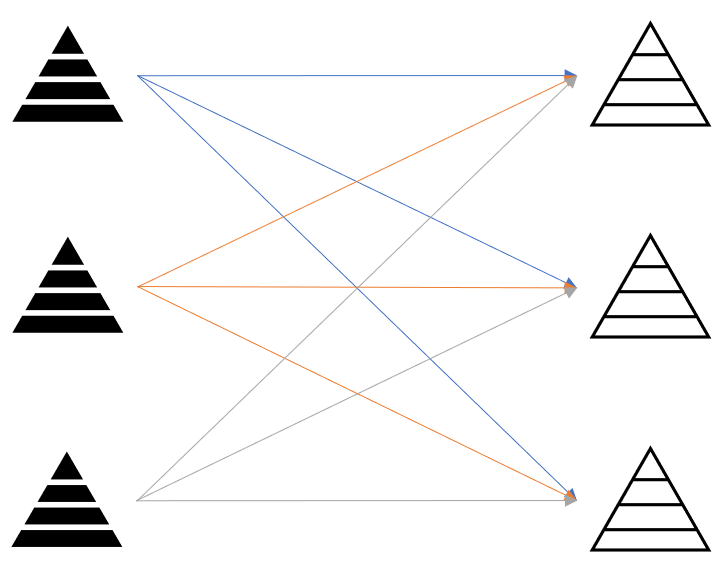
\includegraphics[width=\linewidth]{Identities_complexityQuadratic}
    \caption{Quadratic Complexity}
    \label{fig:Identities_complexityQuadratic}
  \end{minipage}\hfill
  \begin{minipage}{0.48\textwidth}
    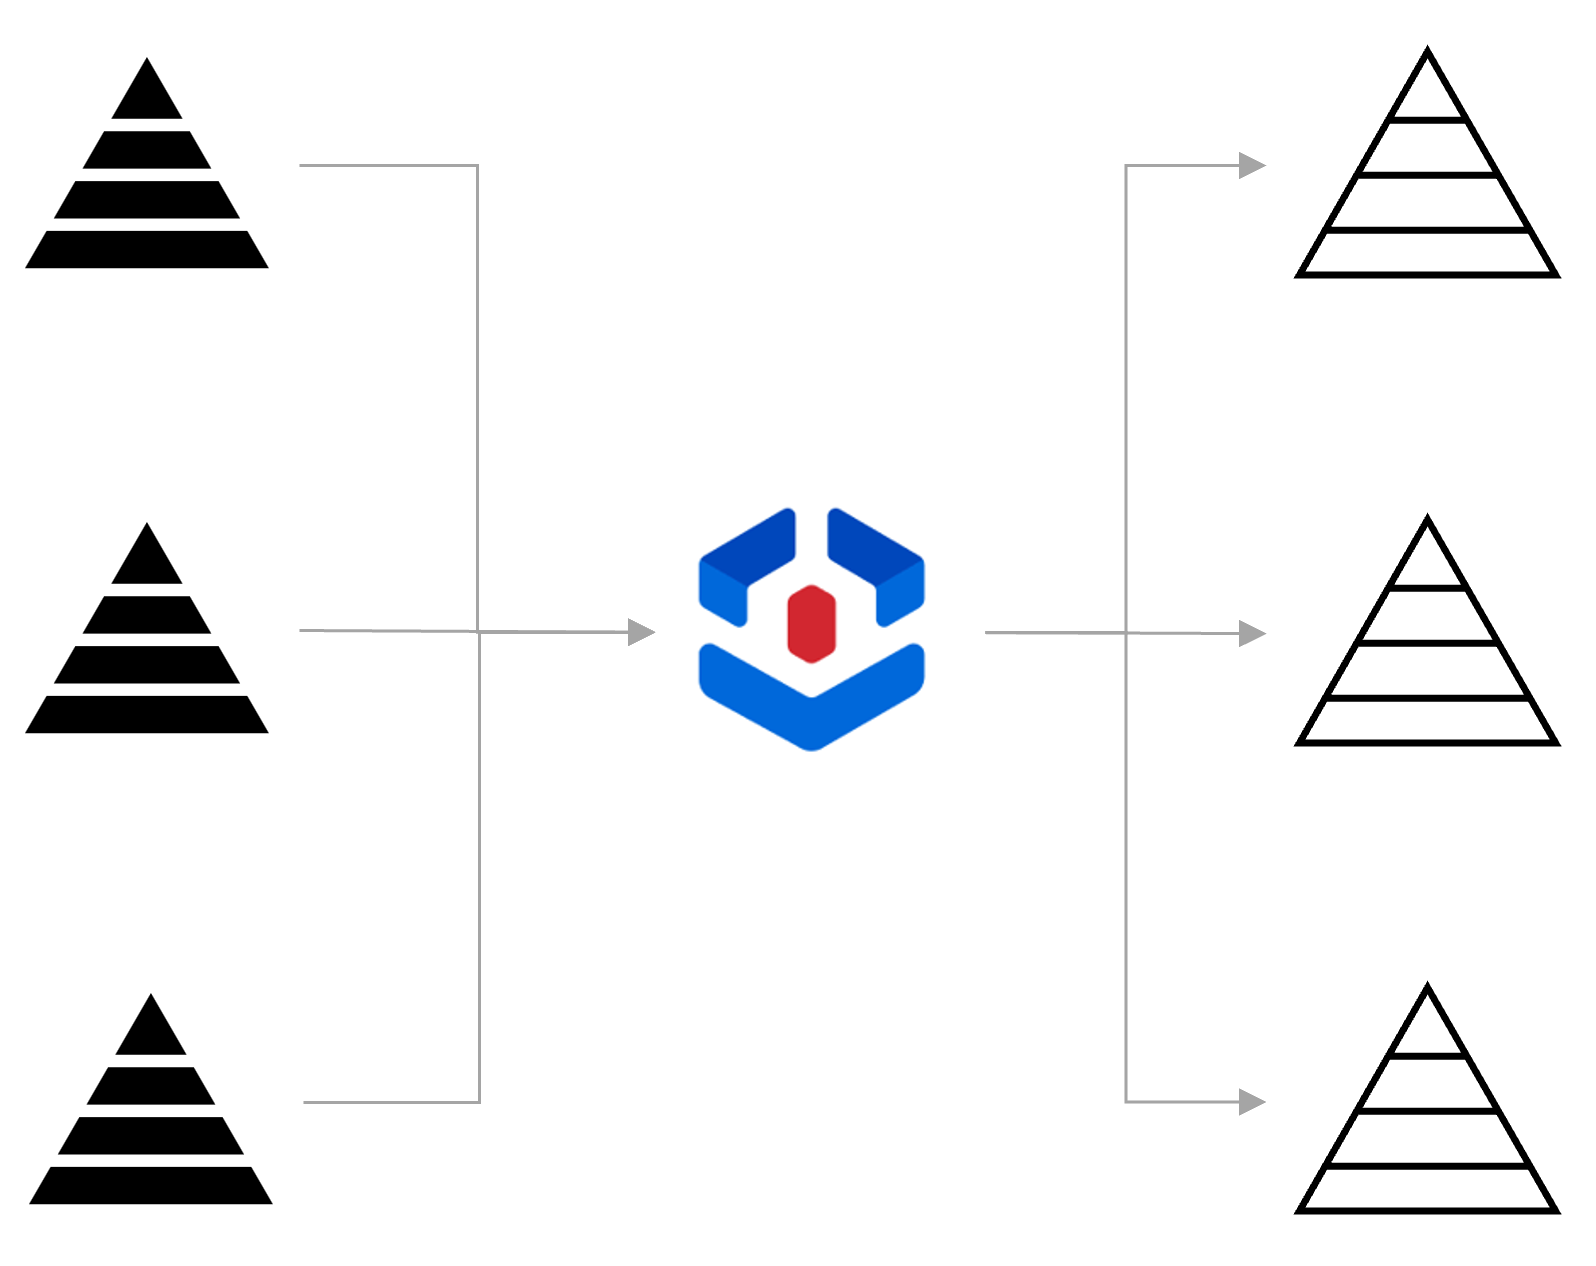
\includegraphics[width=\linewidth]{Identities_complexityLinear}
    \caption{Linear Complexity}
    \label{fig:Identities_complexityLinear}
  \end{minipage}
\end{figure}


\subsection{Entitlement Management}


The process of managing identities’ entitlements is a complex task that necessitates the meticulous assignment of entitlements to identities. This task is particularly important in the context of a role model, which is a subset of a policy that includes governance data such as risk definition. The role model is designed to manage entitlements across all managed systems and establish rules that initiate the assignment of these entitlements to identities.

Entitlements in a managed system can take on various forms. They serve as permissions for identities to access specific data on a system or a physical location. For instance, in the Active Directory, entitlements are typically group memberships. To have administrator rights in the Iris application, a user must be a member of the group SGAPPIT/Development/Iris/Administrator.

Usercube is a tool specifically designed to help create a comprehensive and reliable catalog of the entitlements available in the managed systems. It ensures that the appropriate entitlements are assigned to the correct users. The role model in Usercube encompasses the entitlements, represented as roles, for all managed systems. It also includes rules that manage the systems’ resources and initiate the assignment of entitlements to identities.

The role model is part of a broader policy that also includes governance data such as risk definition. This allows for the implementation of distinct behaviors through distinct policies at a higher level.

Usercube represents IGA-related access right mechanisms through a role-based model. The role catalog aims to contain a comprehensive list of entitlements from all managed systems. Each entitlement is modeled by a role, and NETWRIX recommends creating a single role for each entitlement with a name that is more functional than technical for easy understanding.

Roles alone are not sufficient to provide identities with the systems’ technical entitlements. Rules are needed for Usercube to write users’ entitlements in the managed systems. These rules are used to automatically assign roles to users and categorize users and accounts.

Provisioning rules are a specific type of rule in Usercube. They write the actual entitlements to the managed systems, often based on users’ roles. For example, to give an AD entitlement to a user, a rule is needed that adds the user to the member list of a specific AD group when a specific role is assigned to them. Even when a role is manually assigned, provisioning rules determine which account and permission groups are given as entitlements.

While the role catalog and provisioning rules are together enough to manually give users their access rights, we often want Usercube to do this automatically. Assignment rules automatically assign roles to identities based on specific criteria. For example, we can choose to assign the role Benefits Manager - FR to any user whose job title is benefits manager and whose location is in France.

Once all assignment rules are created, Usercube is able to spot existing assignments that are not supported by any rule, marking them as non-conforming.

Usercube’s assignment rules include single role rules and composite role rules to assign single and composite roles, and resource type rules to assign accounts.

Different resources can be managed through different rules, by being part of different resource types. A resource type is a group of resources that have the same IGA-related purposes. Categorization rules categorize resources into resource types and link identities to the accounts they own.

For example, we might need to differentiate AD’s standard accounts from administration accounts. This way, we can configure different email addresses for privileged accounts, for example adm.john.smith@contoso.com. We can also add more approval steps in the workflows related to privileged accounts, for more security than for standard accounts.

\begin{figure}[htbp]
  \centering
  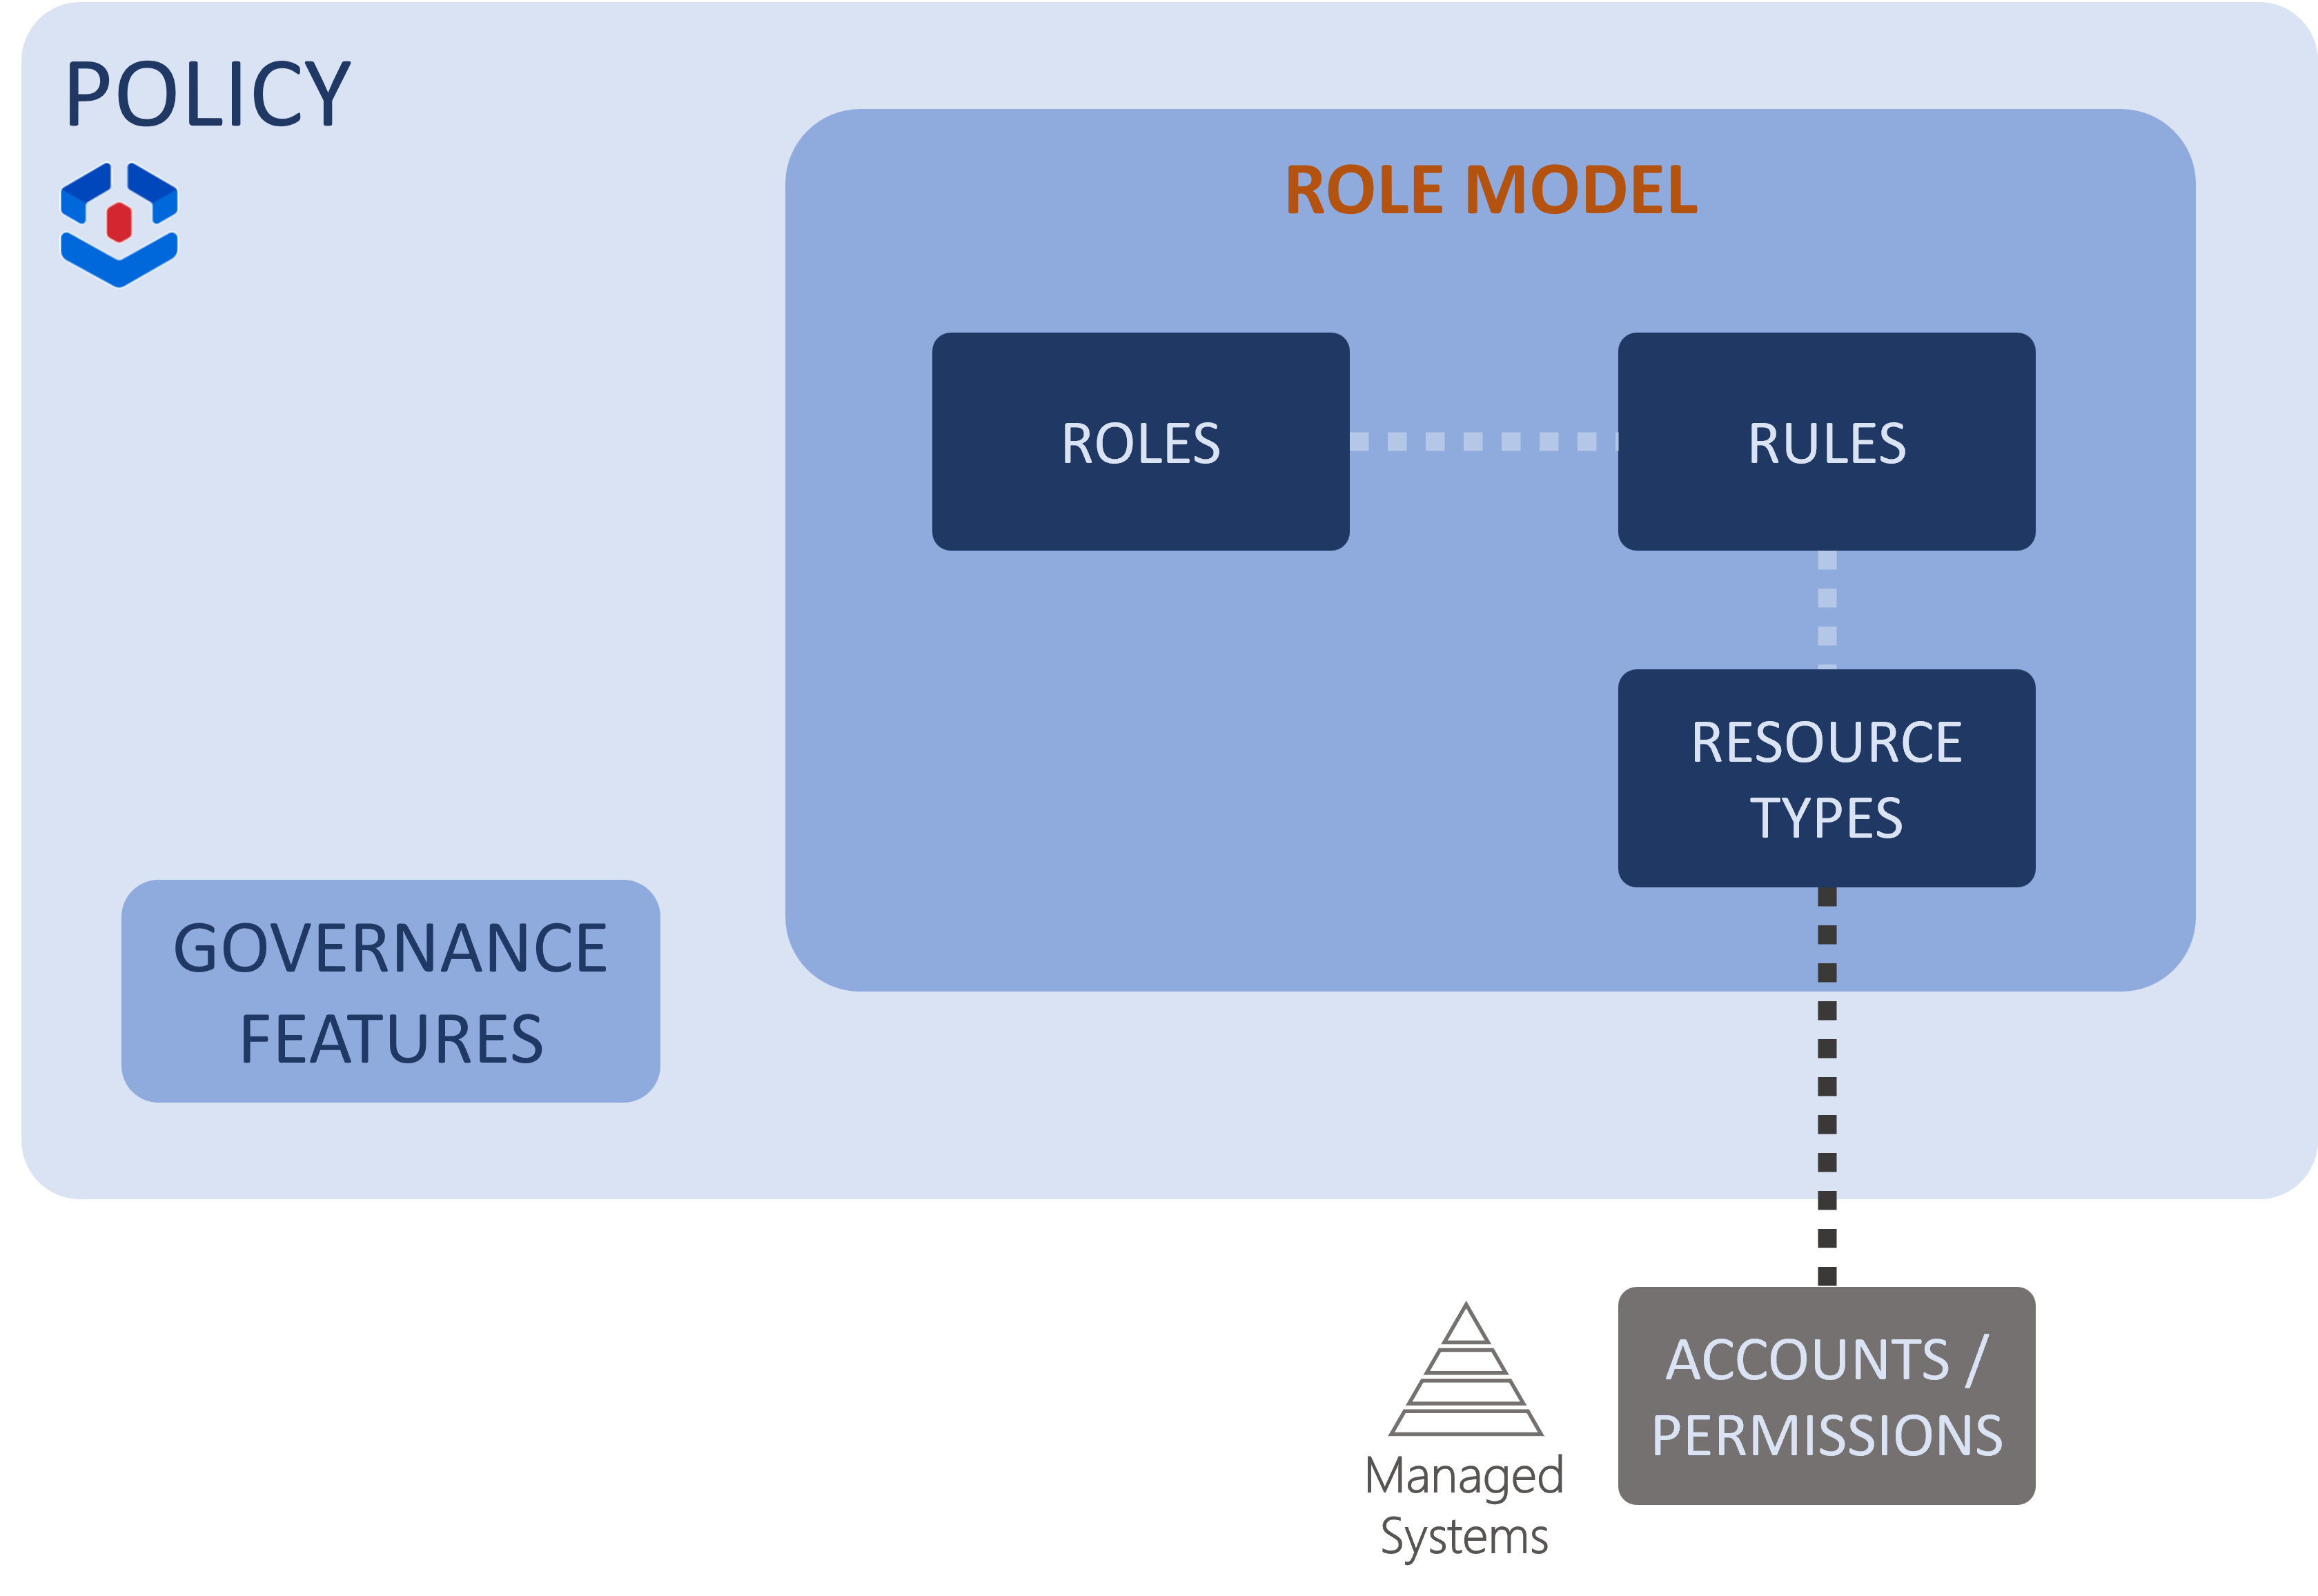
\includegraphics[width=5in]{Entitlements_RoleModel}
  \caption{Entitlements Role Model}
  \label{fig:Entitlements_RoleModel}
\end{figure}



\subsection{Architecture}


Usercube works via a server which operates computation, stores all application data in the database, and serves a web User Interface; at least one agent which operates data flows to/from the managed systems. The managed systems' credentials are used only by the agent and are never disclosed to the server. The agent can call the server, but the server cannot call the agent. The data flows' initiatives are always from the agent. In our case the installation is on-premises so that the server is installed on an isolated network within the company.

\begin{figure}[htbp]
  \centering
  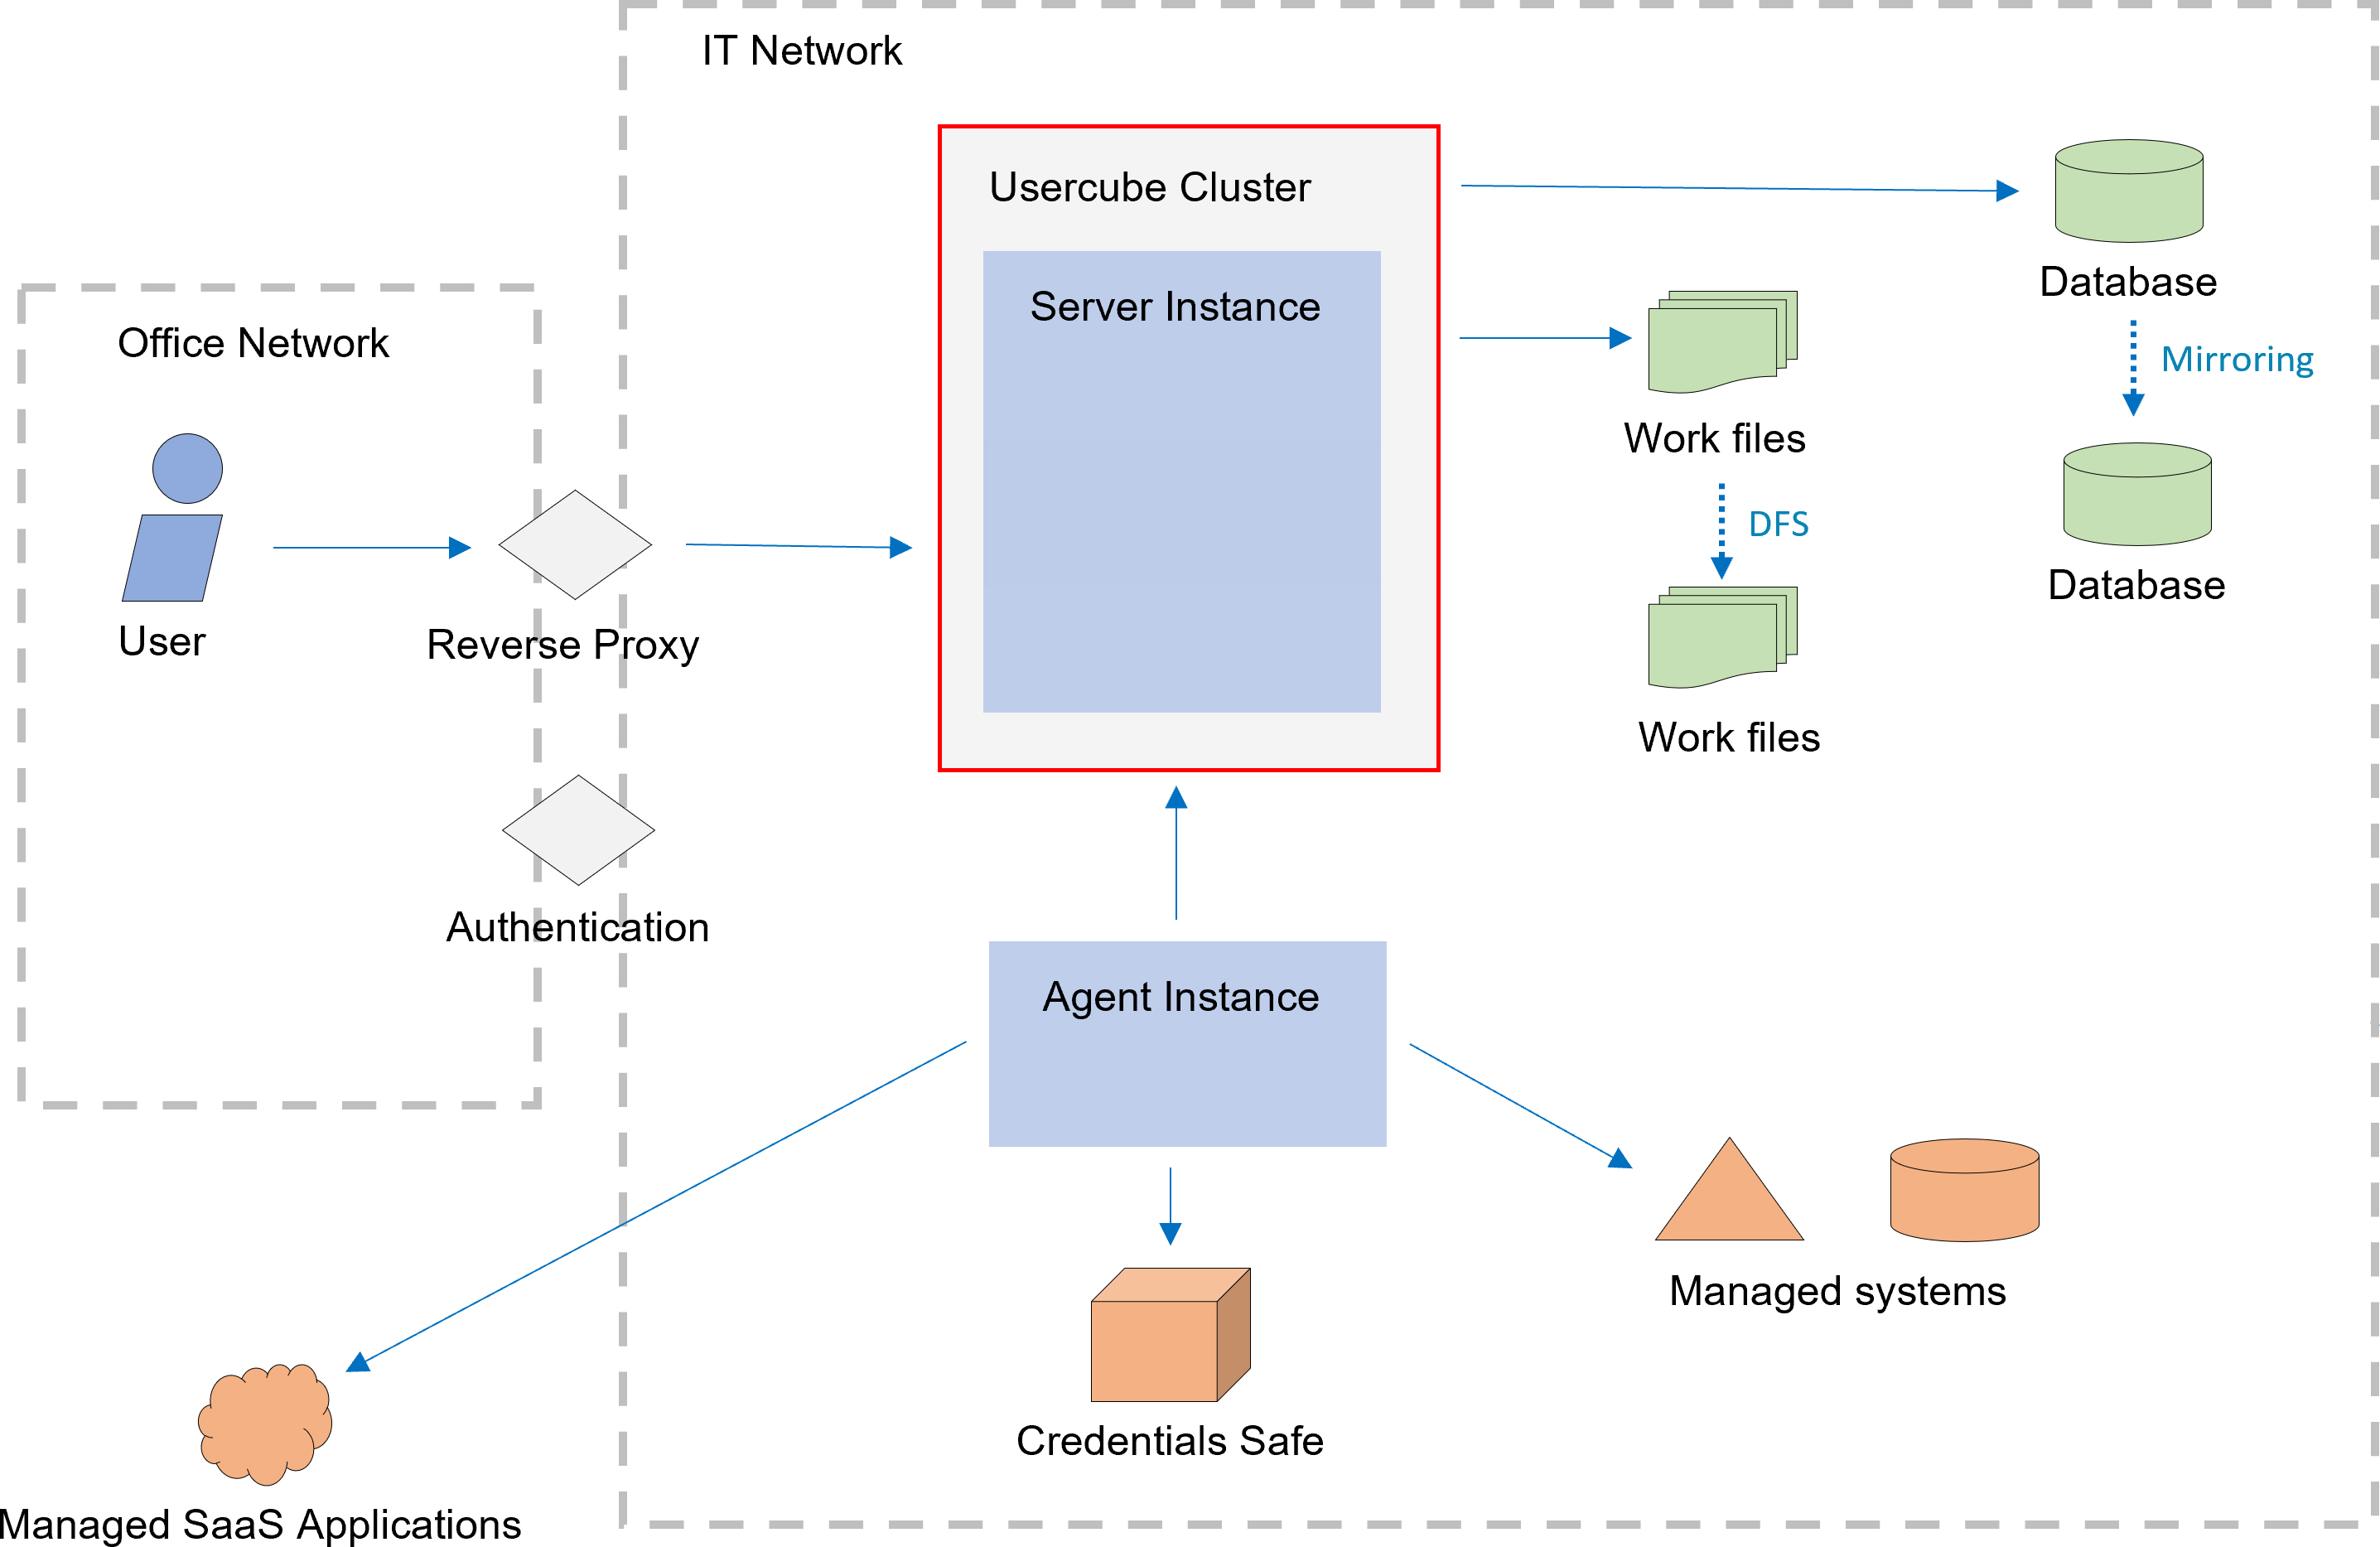
\includegraphics[width=5in]{Architecture_onPrem}
  \caption{Architecture on premises}
  \label{fig:Architecture_onPrem}
\end{figure}

\subsection{Configuration}

A Usercube configuration is a set of XML files edited according the Usercube schema. The recommendations part of this section explains how to set up an editing environment for the configuration.

Regardless of the editing space, the configuration persists in the Usercube database. It's this stored configuration that is used at runtime. The Deploy configuration tool is used to import a new version of the configuration (from the XML files set).

The Export configuration tool can be used to export the current configuration (to a XML files set). The Usercube project's integration cycle consists in developing a configuration by successive imports in a test instance.

The XML configuration schema shows some similarities with the database schema but they are not the same.

\begin{figure}[htbp]
  \centering
  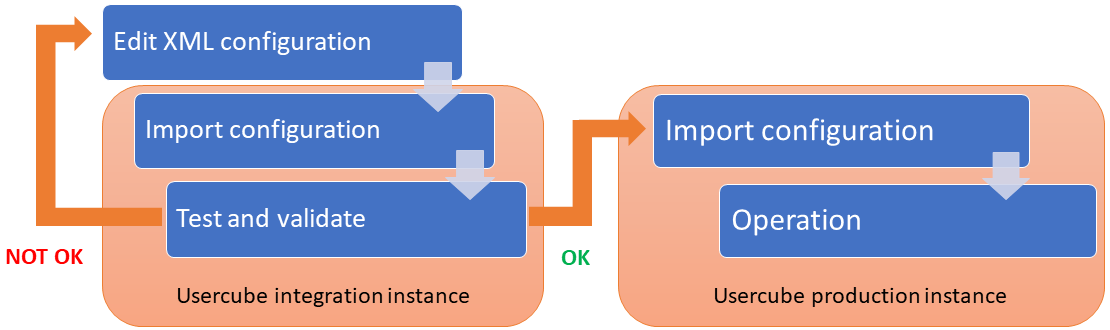
\includegraphics[width=5in]{configurationCycle}
  \caption{Usercube's configuration Cycle}
  \label{fig:configurationCycle}
\end{figure}

\subsection{Testing}


for testing we have different enviroments running in virtual machines. we deploy the new configuration to a testing instance and check if there is initial erros. Then the functional team is the one responsible to test the developments. After the test is done they send us back the ticket and then we save our code to build the next mep

\subsection{Deployment}


Deploy a local XML configuration by using the Deploy-Configuration executable and declaring at least: the configuration directory; the connection string of the database.
